\documentclass[sigconf,anonymous,review]{acmart}
\usepackage{booktabs}
\setcopyright{none}
\acmConference[WSDM '27]{ACM International Conference on Web Search and Data Mining}{February 15--19, 2027}{Hong Kong, China}
\acmYear{2027}
\copyrightyear{2027}
\acmDOI{}
\acmISBN{}

% Generated from independently audited frozen artifacts.
\newcommand{\TCLQueries}{61,763}
\newcommand{\ExposedQueries}{19,533}
\newcommand{\UnchangedQueries}{42,230}
\newcommand{\ExposurePct}{31.63}
\newcommand{\UnchangedPct}{68.37}
\newcommand{\TrainingAP}{0.1350}
\newcommand{\TrainingAccuracy}{0.0803}
\newcommand{\CenteredAP}{0.0971}
\newcommand{\CenteredLow}{0.0925}
\newcommand{\CenteredHigh}{0.1016}
\newcommand{\HistoryAP}{0.00022}
\newcommand{\HistoryAccuracy}{0.00030}
\newcommand{\HistoryExposed}{0.00095}
\newcommand{\PermHistoryExposed}{0.00139}
\newcommand{\TrainingUnchanged}{0.0950}
\newcommand{\TrainingExposed}{0.0485}
\newcommand{\UnchangedMin}{0.0887}
\newcommand{\UnchangedMax}{0.1038}
\newcommand{\OrderingChangesPct}{2.77}
\newcommand{\TrainingPoints}{8.03}
\newcommand{\TrainingUnchangedPoints}{9.50}
\newcommand{\HistoryPoints}{0.03}
\newcommand{\MOOCAdv}{32.67}
\newcommand{\MOOCAdvLow}{32.14}
\newcommand{\MOOCAdvHigh}{33.20}
\newcommand{\MOOCInteraction}{33.90}
\newcommand{\MOOCInteractionLow}{33.18}
\newcommand{\MOOCInteractionHigh}{34.61}
\newcommand{\MOOCOriginalAcc}{45.00}
\newcommand{\MOOCCommonQueries}{60,630}
\newcommand{\MOOCTrainEvents}{227,485}
\newcommand{\WikiAdv}{17.05}
\newcommand{\WikiAdvLow}{16.24}
\newcommand{\WikiAdvHigh}{17.86}
\newcommand{\WikiInteraction}{16.15}
\newcommand{\WikiInteractionLow}{15.41}
\newcommand{\WikiInteractionHigh}{16.89}
\newcommand{\WikiOriginalAcc}{9.90}
\newcommand{\WikiCommonQueries}{14,515}
\newcommand{\WikiTrainEvents}{79,202}
\newcommand{\SignFlipP}{0.000977}
\newcommand{\MOOCUnseenNegativePct}{64.96}
\newcommand{\MOOCSeenAccuracy}{90.32}
\newcommand{\MOOCUnseenAccuracy}{20.55}
\newcommand{\MOOCExcludedMin}{17.46}
\newcommand{\MOOCExcludedMax}{19.29}
\newcommand{\MOOCOriginalAdv}{18.34}
\newcommand{\MOOCCountsOriginalAcc}{33.72}
\newcommand{\WikiUnseenNegativePct}{98.75}
\newcommand{\WikiSeenAccuracy}{93.30}
\newcommand{\WikiUnseenAccuracy}{8.84}
\newcommand{\WikiExcludedMin}{62.88}
\newcommand{\WikiExcludedMax}{66.13}
\newcommand{\WikiOriginalAdv}{2.43}
\newcommand{\WikiCountsOriginalAcc}{6.35}
\newcommand{\TrainingExposedPoints}{4.85}
\newcommand{\ArchiveWikiTCL}{0.0555}
\newcommand{\ArchiveMOOCTCL}{0.1076}
\newcommand{\ArchiveLastFMTCL}{0.2423}
\newcommand{\ArchiveLastFMDyG}{0.0019}
\newcommand{\ArchiveLastFMDyGAP}{0.9245}
\newcommand{\ArchiveLastFMTCLAP}{0.7552}
\newcommand{\BothSeenMOOCAdv}{55.00}
\newcommand{\BothSeenWikiAdv}{19.31}
\newcommand{\BothSeenMOOCQueries}{36,009}
\newcommand{\BothSeenWikiQueries}{12,813}
\newcommand{\WikiSeenPositiveUnseenNegativePct}{87.45}

% Retrospective local permutations; recorded_audit/local_permutation_support/RESULT.json
\newcommand{\MOOCWithinBothSeenAcc}{83.69}
\newcommand{\MOOCBetweenBothSeenAcc}{83.80}
\newcommand{\MOOCGlobalBothSeenAcc}{26.97}
\newcommand{\WikiWithinBothSeenAcc}{92.45}
\newcommand{\WikiBetweenBothSeenAcc}{92.48}
\newcommand{\WikiGlobalBothSeenAcc}{73.02}
\newcommand{\DyGTraining}{22.34}
\newcommand{\DyGHistory}{0.38}
\newcommand{\DyGTrainingSeedOne}{22.27}
\newcommand{\DyGTrainingSeedTwo}{22.42}
\newcommand{\DyGHistorySeedOne}{0.37}
\newcommand{\DyGHistorySeedTwo}{0.39}
\newcommand{\DyGExposure}{87.53}
\newcommand{\DyGFlip}{3.93}

\begin{document}
\title{Interpreting Timestamp Permutations in Dynamic Link Prediction}
\author{Anonymous Author(s)}

\begin{abstract}
Timestamp permutations can change both model training and the history supplied at evaluation. Their effects are therefore ambiguous unless these interventions are separated and their reach into model inputs is measured. We cross training chronology with evaluation history to obtain four conditions, A--D, and measure input exposure and within-query discrimination. On MOOC, TCL trained with binary cross-entropy gains 8.03 percentage points in pairwise accuracy from original chronology under common evaluation history, whereas changing history at fixed weights gives a 0.03-point contrast. Suppressing explicit time encodings during both training and inference reduces the training contrast to 3.64 points; the paired reduction is 4.39 points [3.68, 5.09] across six seeds. A two-seed DyGFormer comparison on the same queries yields a \DyGTraining{}-point training contrast and \DyGHistory{}-point history contrast, with substantially greater input exposure. Matched logistic controls further establish chronology-dependent recency utility under historical and random negative sampling on MOOC. These results distinguish training-procedure sensitivity, explicit-feature dependence, and response to altered evaluation inputs, providing a practical protocol for interpreting permutation experiments.
\end{abstract}
\ccsdesc[500]{Information systems~Data mining}
\ccsdesc[300]{Computing methodologies~Machine learning}
\keywords{temporal graphs, dynamic link prediction, evaluation, timestamp permutation}
\maketitle

\section{Introduction}
A drop in dynamic link-prediction performance after permuting timestamps is often taken as evidence that a model learned useful temporal information~\cite{rahman2025counterfactual}. The interpretation depends on the intervention. Retraining on permuted events can change temporal features, neighborhoods, update order, optimization, and checkpoint selection. Changing the history supplied to a trained model instead measures its response to different evaluation inputs. A small history effect has another explanation: a bounded neighborhood may never contain the altered events.

Predictive quality alone does not resolve these alternatives. EdgeBank demonstrates the strength of edge memorization and the influence of negative sampling~\cite{poursafaei2022towards}; recency and popularity heuristics can compete with neural models~\cite{cornell2025heuristics}. Benchmarks and common implementations improve comparability~\cite{tgb2023,yu2023dygformer}, but an architectural ranking does not identify sensitivity to chronological organization. Removing time encoding is a different intervention again: it changes the learned system, rather than separating training chronology from evaluation history.

Related temporal-sensitivity studies examine trained predictors on temporally distorted test data~\cite{rahman2025counterfactual}, graph characteristics and timestamp granularity~\cite{hayes2025learn}, and generated graphs with known causal structure~\cite{rahman2026causal}. We address the interpretation of a permutation comparison itself. Crossing training and history separates two contrasts; comparing actual inputs establishes which queries are exposed to the history intervention. An explicit-feature ablation then tests how a training contrast depends on time encoding.

We ask: (i) does original training improve discrimination under common evaluation history; (ii) how does explicit time encoding modify this contrast; and (iii) how do input exposure and candidate construction shape permutation sensitivity? Our contribution is a crossed, exposure-aware diagnostic, a six-seed TCL-BCE study with matched time-encoding ablation, and an architectural transfer to DyGFormer. Logistic controls examine recency under matched candidate protocols. The resulting evidence concerns specified training procedures and inputs; the diagnostic does not equate a permutation gap with a unique internal temporal-reasoning mechanism.

\section{Diagnostic Design}
\subsection{Crossing training chronology and history}
An interaction consists of two endpoints, an event time, and associated features. Dynamic link prediction uses preceding interactions to rank an observed pair against a sampled alternative at a fixed query time. We freeze the chronological split and node-exclusion rule before intervention. On MOOC, each permutation reassigns timestamps among the 288,224 history events before the split boundary while preserving each event's endpoints and features. The same 227,485 events satisfying the node-exclusion rule supply training examples. Events involving excluded nodes can still enter evaluation history. Validation/test events, query times, and evaluation candidates remain fixed.

Let $\theta_{s,0}$ and $\theta_{s,\pi}$ denote selected weights trained with original and permuted chronology for training seed $s$ and permutation $\pi$. Let $H_0,H_\pi$ denote evaluation histories. History contains only events strictly preceding each query; $H_\pi$ changes the training prefix while later observed events retain their original times. Define
\[
 A=M(\theta_{s,0},H_0),\quad B=M(\theta_{s,0},H_\pi),
\]
\[
 C=M(\theta_{s,\pi},H_0),\quad D=M(\theta_{s,\pi},H_\pi).
\]
Each selected model is evaluated under both histories without retraining. A--C is the \emph{training-procedure contrast}: evaluation history is common, while training features, neighborhoods, optimization, and model selection can differ. A--B and C--D are history contrasts at fixed original-trained and permutation-trained weights. Their interaction,
\begin{equation}
 I=(A-B)-(C-D),
\end{equation}
measures how the history response depends on training chronology. A--D changes both factors and cannot substitute for these separate contrasts.

\begin{table*}[t]
\centering\small
\caption{Crossed MOOC diagnostic. A--D are pairwise accuracies (\%); contrasts are percentage points. TCL-BCE rows average five permutations within each of six seeds, then average seeds. DyGFormer rows report the two seeds separately, each averaging five permutations. ON/OFF refers to explicit time encoding during training and inference. AP, centered AP, individual permutations, and seed-level intervals are in the artifact.}
\label{tab:crossed}
\begin{tabular}{@{}llrrrrrrrr@{}}
\toprule
Configuration & Seeds & A & B & C & D & A--C & A--B & C--D & $I$\\
\midrule
TCL-BCE ON & 6 & 81.90 & 81.87 & 73.87 & 73.92 & 8.03 & 0.03 & -0.04 & 0.07\\
TCL-BCE OFF & 6 & 70.00 & 69.92 & 66.36 & 66.39 & 3.64 & 0.08 & -0.03 & 0.11\\
\midrule
DyGFormer & 1004 & 86.90 & 86.54 & 64.64 & 64.37 & 22.27 & 0.37 & 0.27 & 0.10\\
DyGFormer & 1005 & 86.95 & 86.57 & 64.54 & 64.29 & 22.42 & 0.39 & 0.24 & 0.14\\
\bottomrule
\end{tabular}

\end{table*}

\subsection{Input exposure and prediction quality}
For each query, compare the tensors supplied under $H_0$ and $H_\pi$ for the source and both candidates. For TCL-BCE these include ordered node/edge features, time differences, and padding masks. A query is exposed if any compared input changes. The unchanged-input group has identical inputs across all tested histories. At fixed weights, equal inputs imply equal predictions up to numerical precision. This is a property of intervention reach, not a claim about responses to changes that never reach the model.

We report pooled average precision (AP) and pairwise accuracy, which credits one when the positive candidate ranks above the negative and one half for a tie. AP ranks examples across queries, while pairwise accuracy isolates within-query discrimination. As an additional diagnostic, subtract each query's mean of its two logits from both logits and recompute pooled AP. This label-free centering preserves every within-query ranking and removes a shared additive query offset; it is not an additive decomposition of AP.

\section{Experiments and Findings}
\subsection{Controlled TCL-BCE evaluation}
We use the TCL architecture~\cite{wang2021tcl} in a DyGLib-based implementation~\cite{yu2023dygformer}, trained with binary cross-entropy; we call this configuration \emph{TCL-BCE}. MOOC records learner--resource interactions~\cite{kumar2019jodie}. Evaluation covers all \TCLQueries{} test queries with one fixed random negative per query, including 670 positive--negative candidate collisions. Each endpoint selects its 20 most recent preceding interactions.

For each of six seeds (1004--1009), we train on original chronology and five permutations, giving 36 selected models. Adam training uses 20--100 epochs, patience 10, and the earliest strict maximum of pooled validation AP for checkpoint selection. Reusing the original model across its five permutations gives 96 unique evaluation panels. We average permutation contrasts within each seed; descriptive 95\% $t_5$ intervals use the six seed means, not queries or repeated A cells, as their uncertainty units.

\subsection{Training and history have different effects}
Under common original history, A--C is 8.03 accuracy points [7.65, 8.41] and 13.50 AP points [12.56, 14.44]. The centered-AP contrast remains 9.71 points [9.25, 10.16], positive for every seed, while all within-query rankings are preserved by centering. Thus the advantage includes better within-query discrimination and is not explained entirely by additive offsets between queries. Excluding the 670 candidate collisions leaves 61,093 queries, with an 8.11-point accuracy contrast [7.73, 8.50] and a 13.83-point AP contrast [12.86, 14.79].

The history-only A--B contrast is 0.03 accuracy points. Each permutation changes the same 19,533 queries (31.63\%); the other 42,230 have identical inputs across all tested histories. Unchanged validation and earlier test interactions can displace altered training events from bounded histories. Exposure falls from 39.15\% in the first equal-count test decile to 14.04\% in the last. Only 6.85--6.88\% of eligible timestamp-altered TRAIN events occur in the selected test neighborhoods.

\begin{figure*}[t]
\centering
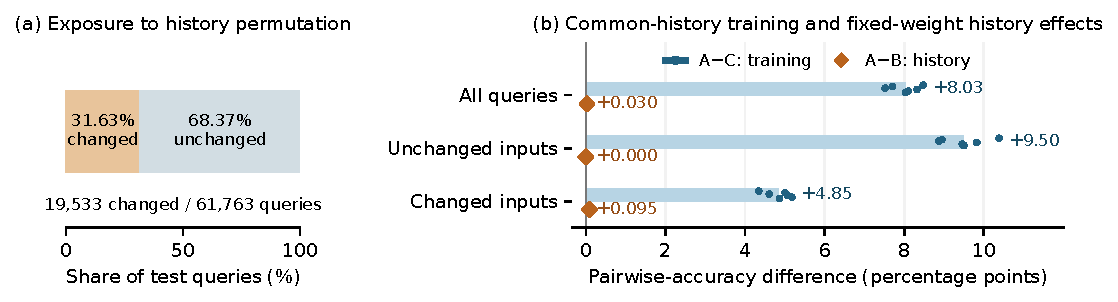
\includegraphics[width=\textwidth]{diagnostic.pdf}
\caption{TCL-BCE: history exposure and training/history contrasts. (a) Queries with changed or identical inputs across tested histories. (b) Pairwise-accuracy differences in points: blue bars are A--C means, dots are six seed means, and orange diamonds are A--B means at fixed original-trained weights. Five permutations are first averaged within seed. Input-defined groups differ in composition.}
\Description{31.63 percent of queries have changed inputs. Training contrasts are 8.03 points overall, 9.50 for unchanged inputs and 4.85 for changed inputs; history contrasts are about 0.03, zero and 0.095 points.}
\label{fig:diagnostic}
\end{figure*}

Exposure is only part of the explanation. Among exposed queries, 2.77\% change candidate ordering; opposing gains and losses leave an A--B contrast of 0.095 points, while C--D is $-0.139$ points. Unchanged inputs produce no history-induced ranking flips in either training condition. Their maximum logit drift across 60 fixed-weight comparisons is $6.63\times10^{-6}$, within the prespecified tolerance $2\times10^{-5}+10^{-5}(|z_0|+|z_\pi|)$. The interaction is 0.074 points [0.023, 0.125]. A small aggregate history effect therefore combines limited exposure, stable rankings, and cancellation.

A--C remains 9.50 points on unchanged-input queries and 4.85 points on exposed queries (Figure~\ref{fig:diagnostic}), with positive seed means in both groups. Common evaluation history already excludes immediate history differences as the source of A--C; the unchanged-input analysis additionally locates the advantage where the tested history interventions leave model inputs untouched. The groups are descriptive, not randomized strata for a causal moderation claim.

\subsection{Explicit time encoding modifies the training contrast}
We repeat the crossed design with the time encoder's output set to zero during both training and inference. The encoder module and parameter layout remain in place; architecture, neighborhood construction, timestamp sorting, candidate rules, and checkpoint-selection rule are otherwise preserved. The ON/OFF comparison contains 72 selected models and 192 unique test panels. A validation pilot with three seeds and two permutations screened the ablation before the six-seed, five-permutation evaluation; its nine OFF models are reused under the same configuration.

With encoding OFF, original-history accuracy is 70.00\% after original training and 66.36\% after permuted training (Table~\ref{tab:crossed}). The training contrast falls from 8.03 to 3.64 points [2.91, 4.37]. Define
\[
\Delta_{\rm time}=(A-C)_{\rm ON}-(A-C)_{\rm OFF}.
\]
The paired reduction is 4.39 points [3.68, 5.09], positive for all six seeds; the contrast is 54.7\% smaller without explicit time encoding. Removing candidate collisions gives a 4.43-point reduction [3.72, 5.15]. AP and centered AP give positive paired reductions of 7.49 and 4.97 points. This intervention establishes that explicit time encoding materially changes chronology sensitivity in this configuration. It does not partition the ON effect into independent mechanisms: suppression also changes the learned predictor, and the remaining contrast can involve temporal neighborhoods, update order, and optimization.

\subsection{Architectural transfer to DyGFormer}
We apply A--D to DyGFormer~\cite{yu2023dygformer} on exactly the same MOOC split, test query IDs, and positive/negative candidates. The comparison uses the complete two-seed A6000 block (1004, 1005), with original training and five permutations per seed: 12 selected models and 32 unique test panels. The block is defined by execution hardware, not by test-effect size. Training uses binary cross-entropy, the same validation selection rule and epoch limits, and DyGFormer's configured 256-event input sequences with patch size eight. Its two-seed, two-permutation validation pilot preceded test evaluation. We report both seed means rather than treating their ten permutation pairs as independent replicates.

The A--C accuracy contrasts are \DyGTrainingSeedOne{} and \DyGTrainingSeedTwo{} points; A--B is \DyGHistorySeedOne{} and \DyGHistorySeedTwo{} points (Table~\ref{tab:crossed}). Thus both seeds show a training contrast larger than the fixed-weight history contrast. DyGFormer's input trace includes node/edge/time features, padding, and neighbor co-occurrence counts; hashes are compared only at fixed weights. The history intervention exposes \DyGExposure{}\% of queries, compared with 31.63\% for TCL-BCE, and changes candidate ordering for \DyGFlip{}\% of exposed queries under original-trained weights. Equal inputs preserve rankings in every checked comparison. Excluding candidate collisions retains the positive training contrast in both seeds. The diagnostic therefore transfers across architectures while revealing distinct exposure and history-response profiles; it is the within-architecture contrasts, rather than absolute model rankings, that support this comparison.

\subsection{Recency under matched candidate protocols}
Full-batch logistic controls separate recency-feature utility from neural architectures and sequential SGD order. A counts/seen baseline uses $\log(1+n)$ for the pair, source, and destination, with three corresponding seen indicators. Adding ages supplies $\log(1+\mathrm{age}/\tau)$ for time since last occurrence, zero when unseen; $\tau$ is the median positive gap between distinct TRAIN times. Both feature sets share their first six columns. Standardization uses TRAIN only; L2 logistic regression uses $C=1$, L-BFGS tolerance $10^{-7}$, and at most 500 iterations.

Original and permuted fits share training query IDs, row order, negative identities, and original causal evaluation history. Historical TRAIN negatives are destinations previously observed with the source in all compared histories, excluding the positive. Empty intersections exclude the query from every fit but preserve its event in history. Random negatives are sampled uniformly from the fixed TRAIN destination universe, excluding the positive, on exactly the same retained queries. Historical test negatives are strictly preceding destinations for the source; random test negatives use the same fixed universe. Both protocols use a common restricted population of 60,630 MOOC and 14,515 Wikipedia queries, excluding absent historical alternatives and archived candidate collisions. Candidate identities remain fixed within each chronology contrast; changing the protocol changes the prediction task.

Let $\Delta_{\rm ages}$ and $\Delta_{\rm counts}$ be original-minus-global-permutation accuracy contrasts, and $\Delta_{\rm recency}=\Delta_{\rm ages}-\Delta_{\rm counts}$. Across ten paired draws, historical negatives yield positive recency contrasts on MOOC (33.90 points [33.18, 34.61]) and Wikipedia (16.15 [15.41, 16.89]). The random TRAIN/test protocol on MOOC retains a 14.17-point contrast [13.99, 14.35], positive in every draw (Table~\ref{tab:candidates}). A three-draw validation pilot preceded the frozen random-protocol evaluation. This MOOC population passes the recorded composition checks: less than 95\% unseen negatives, at least 1,000 both-seen queries, and accuracy below 95\% for a rule using pair-seen status alone, in every draw. The artifact retains the complete two-dataset protocol grid and composition audit; the random-sampling robustness claim concerns MOOC.

\begin{table}[t]
\centering\small
\caption{MOOC logistic training contrasts (points), with 95\% paired $t_9$ intervals over ten draws. H/R: historical/random negatives in both TRAIN and test. Queries are common across protocols; candidates are fixed within each chronology contrast.}
\label{tab:candidates}
\begin{tabular}{@{}lrr@{}}
\toprule
Dataset / negatives & $\Delta_{\rm ages}$ & $\Delta_{\rm recency}$\\
\midrule
MOOC / H & 32.67 [32.14, 33.20] & 33.90 [33.18, 34.61]\\
MOOC / R & 17.21 [17.06, 17.36] & 14.17 [13.99, 14.35]\\
\bottomrule
\end{tabular}

\end{table}

Windowed controls also preserve high historical both-seen accuracy: 83.69--83.80\% on MOOC and 92.45--92.48\% on Wikipedia. They permute within or between 46 equal-duration TRAIN windows of 11.53 hours on MOOC and 21 windows of 24.64 hours on Wikipedia. Because timestamp displacement and disrupted structure both change, these controls characterize interventions rather than identify a unique temporal scale.

\paragraph{Broader descriptive context.}
A separate 195-pair DyGLib archive spans five architectures and four datasets, using ten-epoch budgets, one training-time permutation, random negatives, and joint validation AP/AUC selection. On LastFM, DyGFormer has original AP 0.9245 and a 0.0019 permutation gap (ten pairs); TCL-BCE has AP 0.7552 and a 0.2423 gap (nine unique pairs). These short-budget results are not pooled with the controlled experiments. They illustrate why predictive quality and permutation sensitivity should be reported separately.

\section{Interpretation and Scope}
The crossed and component interventions answer distinct questions. A--C identifies an advantage of a specified training procedure under common evaluation history. The matched ON/OFF contrast establishes dependence of that advantage on explicit time encoding. Input tracing identifies which queries can contribute to a fixed-weight history effect. DyGFormer demonstrates a different exposure profile under the same evaluation candidates. Logistic controls establish chronology-dependent recency utility across two candidate protocols on MOOC.

These estimates concern the specified implementations, datasets, and candidate populations. TCL-BCE intervals describe six training seeds; the architectural transfer reports two seed means; logistic intervals describe ten paired draws on fixed historical-eligible query populations. The benchmark test data were examined previously, and validation pilots also used the checkpoint-selection split. These are controlled comparisons on established benchmarks, not uncertainty over independently sampled datasets. A component ablation establishes sensitivity to that component's inclusion, rather than identifying a unique internal reasoning process.

For a permutation study, freeze splits, query times, candidates, and model-selection rules; cross training chronology with history; measure actual input changes and ranking flips; and aggregate paired contrasts within seeds before reporting uncertainty. Add a matched component or feature control when attributing the training contrast. This protocol turns an undifferentiated permutation gap into testable statements about learning conditions, feature dependence, and evaluation exposure.

\section{Conclusion}
Training chronology and evaluation history are different interventions. Their crossed analysis reveals a substantial training contrast for TCL-BCE, a reproducible reduction when explicit time encoding is suppressed, and architecture-dependent exposure in DyGFormer. Recency controls show that useful chronological organization persists across candidate protocols on MOOC. Reporting training, history, interaction, and exposure together makes permutation results more informative than a single original-versus-shuffled score.
\label{sec:mainend}
\clearpage
\section*{Ethical Considerations}
This study reuses public interaction benchmarks and reports aggregate model behavior. Reproducibility materials preserve pseudonymous identifiers and should respect source-data licenses without releasing additional identifying information. No individual-level behavioral claims are made. The diagnostic distinguishes measured protocol effects from claims about internal mechanisms or deployment performance. AI assistance was used for writing and analysis code; reported quantities were checked against recorded experimental artifacts.
\balance
\bibliographystyle{ACM-Reference-Format}
\bibliography{references}
\end{document}
